\documentclass{beamer}
\usepackage[utf8]{inputenc}
\usepackage{verbatim}
\usepackage{tikz}
\usepackage{hyperref}
\setbeamertemplate{footline}[frame number]
\title{Visualizing Data in R}
\author{\texorpdfstring{Heide Jackson \newline\url{heidej@umd.edu}}{Author}}
\institute{University of Maryland Population Research Center}

\date{August 2019}

\begin{document}
\maketitle
\begin{frame}{High Level Things to Know}
\begin{itemize}
\item R makes it very easy to make very cool graphics.
\item This functionality is available in base R and with the addition of other packages like ggplot2.
\item This presentation will show simply what can be done in Base R without additional packages.
\item Results from R models can often be easily plotted to visually interpret results and diagnose issues in model fit.
\end{itemize}
\end{frame}


\begin{frame}[fragile]{A Simple Graph}
\begin{verbatim}
x<-1:100
y<-100:1
plot(x,y)
\end{verbatim}
\end{frame}

\begin{frame}[fragile]{A simple graph}
\begin{center}
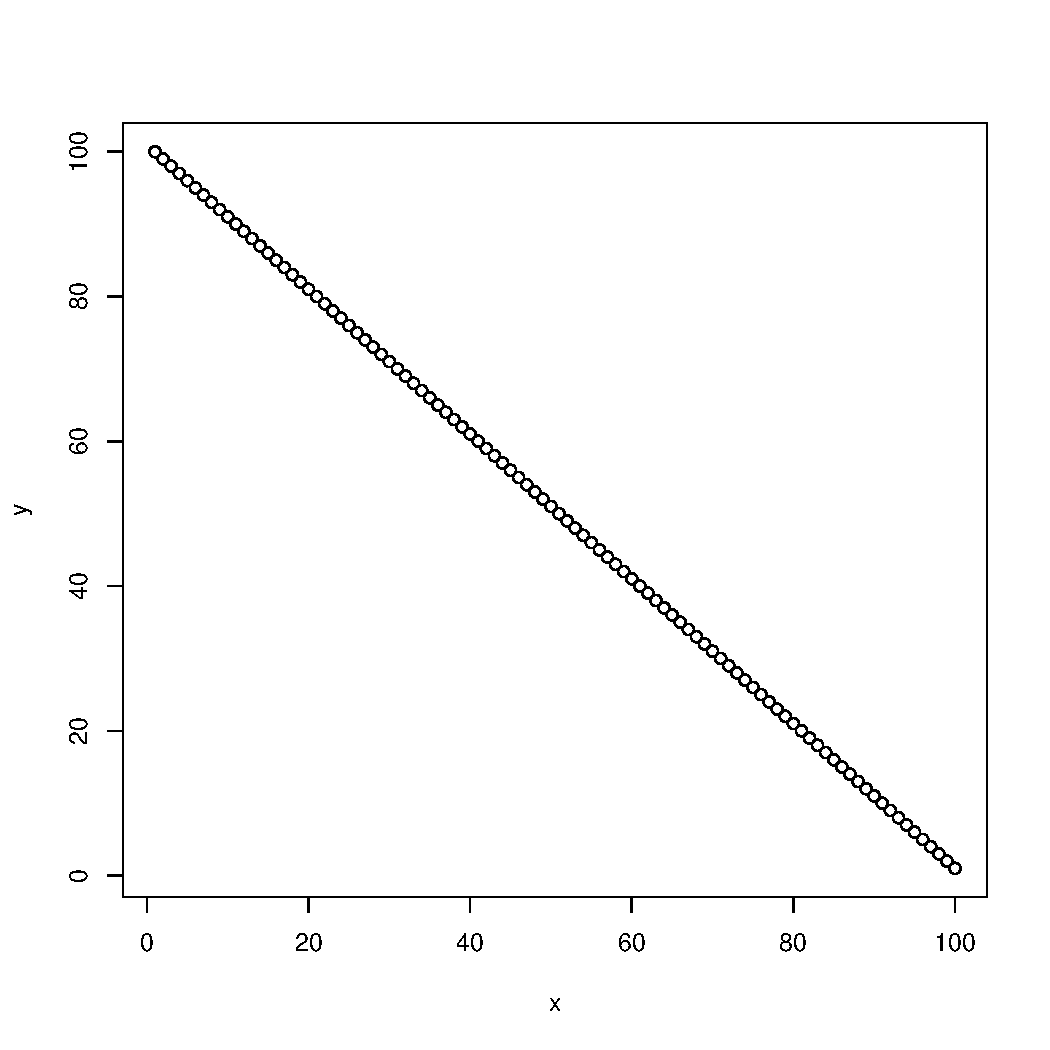
\includegraphics[width=.8\linewidth]{simpleplot.pdf}
\end{center}
\end{frame}
\begin{frame}[fragile]{A simple graph}{Many Options within Plot}
\begin{verbatim}
x<-1:100
y<-100:1
plot(x,y,
ylab="Fancy /n Multiline/n Label", #labels Y axis
xlab="Simple Label", #labels X axis
main="This is a Test", #Graph title
xlim=c(0,100), #Range of X axis
ylim=c(0,100), #Range of Y axis
type="b", #Specify p for point, l for line, or b for both
lty=2, #Type of Line
pch=2, # Type of point, can also be a character in quotes
lwd=3, #specify line thickness
col="red", #Color of plotted objects
bty="l" #Type of box around plot
)
\end{verbatim}
\end{frame}
\begin{frame}[fragile]{A Simple Graph with Options Added}
\begin{center}
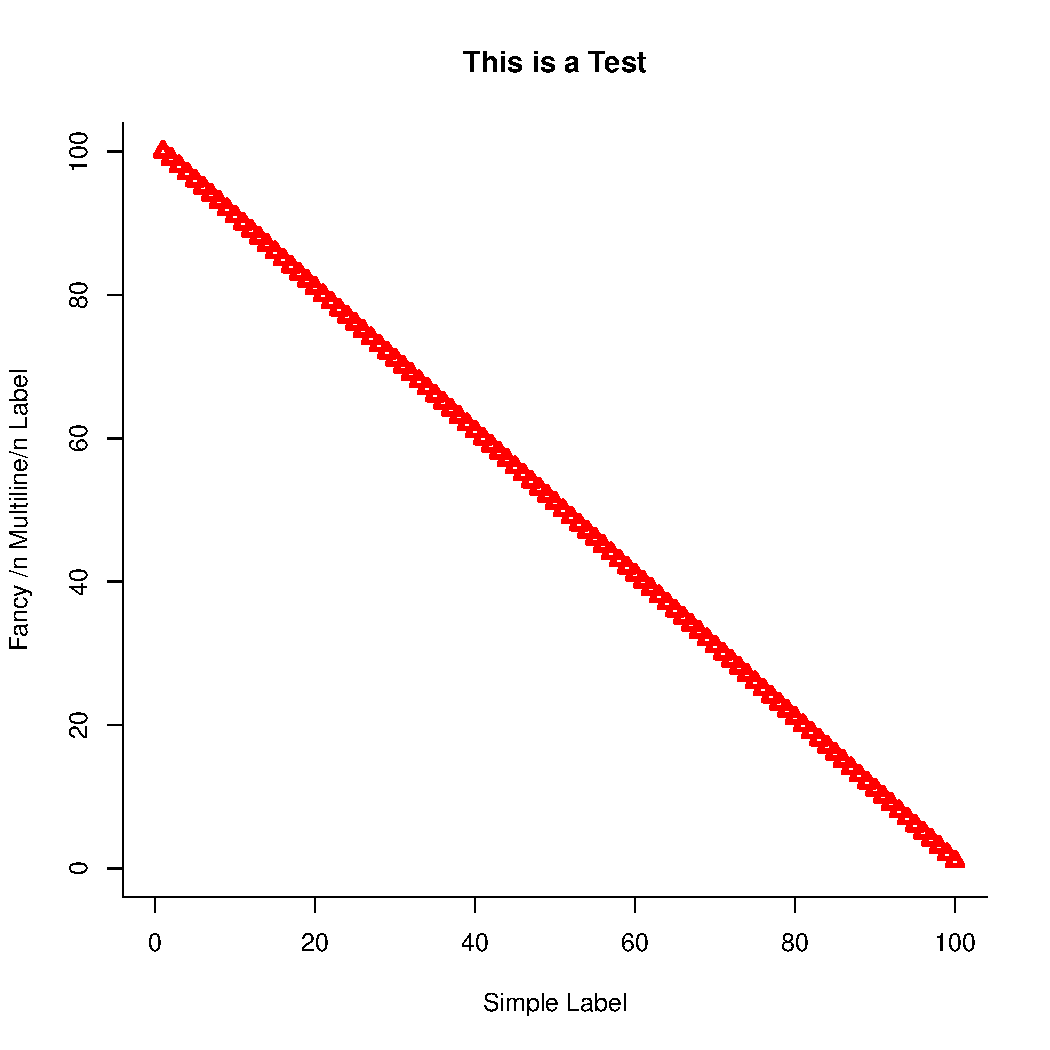
\includegraphics[width=.8\linewidth]{moreoptions.pdf}
\end{center}
\end{frame}
\begin{frame}[fragile]{Adding to the Plot}
\begin{itemize}
\item Plots can be added in multiple steps.  Objects can be overlayed to an initial plot.
\begin{verbatim}
x1<-1:100
y<-100:1
x2<-100:1
plot(x1,y, col="red", type="l")
lines(x2, y, col="blue") #add a line that is blue
points(x1,x2) # add points with these coordinates
legend("topleft", c("Line 1", "Line 2", "Points"), 
col=c("red", "blue", "black"), lty=c(1,1,NA), 
pch=c(NA, NA, 1), bty="n")
\end{verbatim}
\end{itemize}
\end{frame}
\begin{frame}[fragile]{Multi Object Plot}
\begin{center}
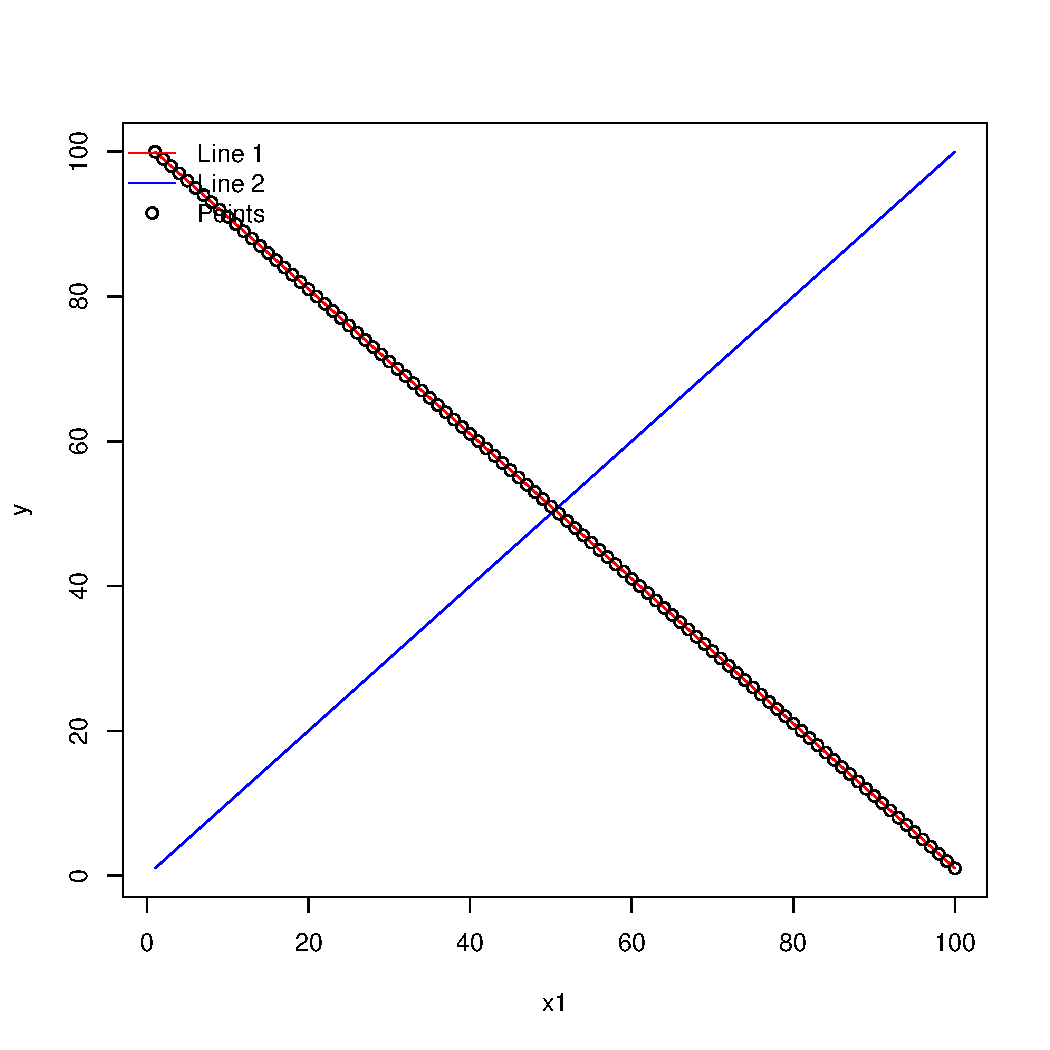
\includegraphics[width=.8\linewidth]{addedoptions.pdf}
\end{center}
\end{frame}

\begin{frame}[fragile]{Adding to the Plot}{Unpacking the Legend}

\begin{verbatim}

legend("topleft", #specify legend location
c("Line 1", "Line 2", "Points"), #Specify labels
col=c("red", "blue", "black"), #Specify object colors
lty=c(1,1,NA), #Specify line type for plotted objects
pch=c(NA, NA, 1), #Specify point types for legend objects
bty="n") # specify if there should be box around legend
\end{verbatim}

\end{frame}


    \begin{frame}[fragile]{Creating a Histogram}

\begin{verbatim}
x1<-rnorm(100,0,1)
y<-100:1
hist(x1)
\end{verbatim}

\end{frame}
\begin{frame}[fragile]{A Histogram}
\begin{center}
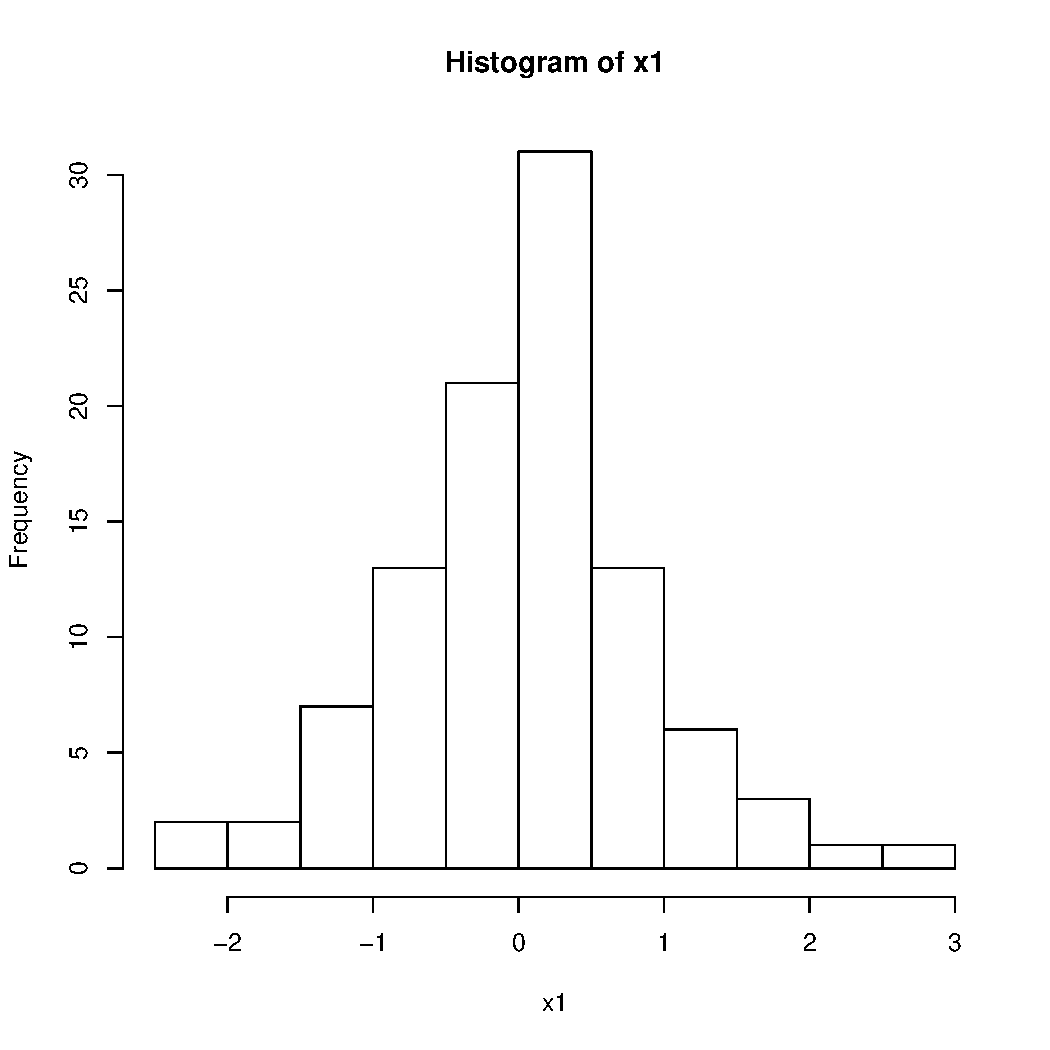
\includegraphics[width=.8\linewidth]{histogram.pdf}
\end{center}
\end{frame}
 
    \begin{frame}[fragile]{Creating a Bar Graph}
    \begin{verbatim}
name=c("Example 1", "Example 2")
x<- c(1,5)
barplot(x, names=name, col=c("red", "blue"))
\end{verbatim}
\end{frame}
\begin{frame}[fragile]{A Bar Graph}
\begin{center}
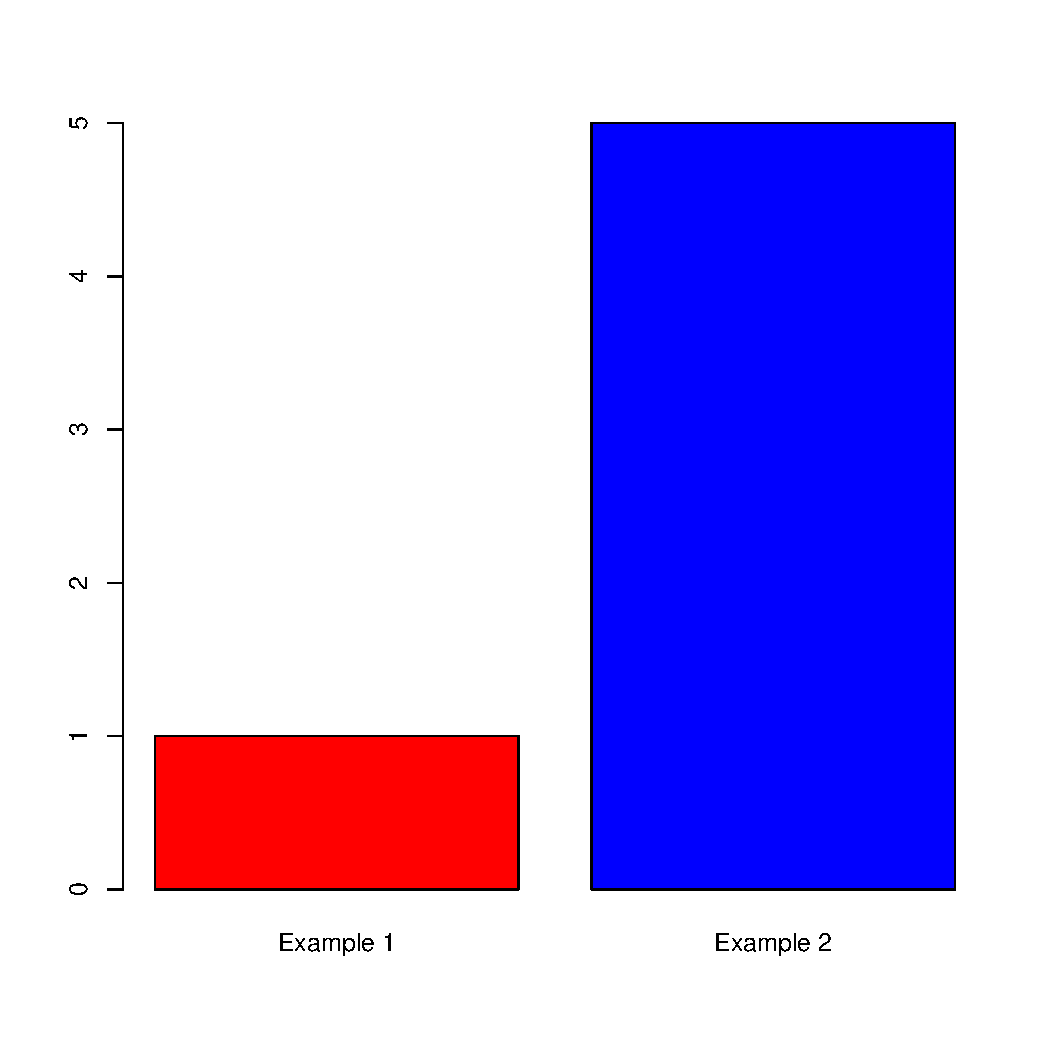
\includegraphics[width=.8\linewidth]{bargraph.pdf}
\end{center}
\end{frame}
\begin{frame}[fragile]{Exporting the Data}
\begin{itemize}
    \item Standard text to export results placed ahead of and after created plot.
    \item R supports many formats but all have a similar syntax. Three I commonly use are pdf(), png(), and tiff()
    \item Here's a quick example:
\begin{verbatim}
    pdf("test.pdf")
    plot(x,y)
    dev.off()
\end{verbatim}
\item Different formats allow for different specification of image size and in some cases resolution--this is particularly useful for posters and journal articles.
\end{itemize}
\end{frame}
\end{document}
